\documentclass[12pt]{article}
\usepackage[paperwidth=25cm,paperheight=17cm,margin=1.5cm]{geometry}
\usepackage[T1]{fontenc}
\usepackage[utf8]{inputenc}
\usepackage[magyar]{babel}
\usepackage{lmodern}
\usepackage{amsmath}
\usepackage{enumitem}
\usepackage{tikz}
\usetikzlibrary{arrows.meta,patterns}

\pagestyle{empty}
\setlength{\parindent}{0pt}
\setlist[enumerate,1]{label=\textbf{\arabic*.}, leftmargin=*, itemsep=4pt, topsep=2pt}
\setlist[enumerate,2]{label=\alph*), leftmargin=2em, itemsep=1pt, topsep=1pt, parsep=0pt}

% Üres ábra képszerkesztéshez: #1 = f, #2 = t, #3 = tárgymagasság
\newcommand{\ures}[3]{%
  \pgfmathtruncatemacro{\gyujto}{#1>0 ? 1 : 0}%
  \draw[gray!25,very thin] (-6,-3.5) grid (7,3.5);
  \draw[->,gray] (-6,0) -- (7.2,0);
  \ifnum\gyujto=1
    \draw[{Stealth[length=2mm]}-{Stealth[length=2mm]},thick,blue!60!black] (0,-3.5) -- (0,3.5);
  \else
    \draw[{Stealth[length=2mm,reversed]}-{Stealth[length=2mm,reversed]},thick,blue!60!black] (0,-3.5) -- (0,3.5);
  \fi
  \fill (#1,0) circle (2pt) node[below,font=\scriptsize] {$F$};
  \fill (-#1,0) circle (2pt) node[below,font=\scriptsize] {$F$};
  \draw[very thick,-{Stealth[length=2mm]}] (-#2,0) -- (-#2,#3);
}

\begin{document}

\begin{center}\vspace*{-0.4cm}
  {\Large\bfseries Geometriai optika -- feladatok}\\[4pt]
  \fbox{\parbox{0.62\textwidth}{\centering
    $c = 3\cdot 10^8~\tfrac{\text{m}}{\text{s}}$, \qquad
    $n_\text{víz} = 1{,}33$, \qquad $n_\text{üveg} = 1{,}5$, \qquad $n_\text{levegő} \approx 1$}}
\end{center}

\begin{enumerate}
\item \textbf{Fénytörés a vízen.} Egy zöld lézer ($\lambda = 532$~nm) fénye levegőből
  $50^\circ$-os beesési szögben éri a víz felszínét.
  \begin{enumerate}
    \item Mekkora a törési szög és a fény sebessége a vízben? Mekkora a fény frekvenciája
      és hullámhossza a vízben? Milyen színűnek látja egy búvár?
    \item Mekkora szöget zár be egymással a visszavert és a megtört sugár?
    \item Egy víz alatti lámpa fénye $40^\circ$-os beesési szögben éri a felszínt alulról.
      Mekkora szögben lép ki a levegőbe?
  \end{enumerate}
\end{enumerate}

\begin{minipage}[t]{0.70\linewidth}\vspace{0pt}
\begin{enumerate}[start=2]
\item \textbf{Lámpa a medence alján.} Egy $1{,}8$~m mély medence alján egy kicsi lámpa
  világít.
  \begin{enumerate}
    \item Mekkora a víz--levegő határszög?
    \item A lámpa fénye a felszínnek csak egy kör alakú részén jut ki a levegőbe. Mekkora
      ennek a körnek a sugara? Mi történik a körön kívülre eső sugarakkal?
    \item Egy búvár a medence fenekéről ferdén felnéz a felszínre, a körön kívüli részre.
      Mit lát ott?
  \end{enumerate}
\end{enumerate}
\end{minipage}\hfill
\begin{minipage}[t]{0.27\linewidth}\vspace{0pt}\centering
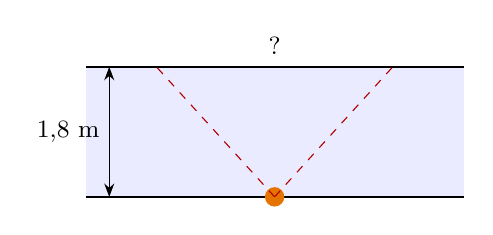
\begin{tikzpicture}[x=0.75cm,y=0.75cm,font=\small]
  \fill[blue!8] (-3.2,-2.2) rectangle (3.2,0);
  \draw[thick] (-3.2,0) -- (3.2,0);
  \draw[thick] (-3.2,-2.2) -- (3.2,-2.2);
  \fill[orange!90!black] (0,-2.2) circle (3.5pt);
  \draw[<->,>=Stealth] (-2.8,-2.2) -- node[left] {$1{,}8$~m} (-2.8,0);
  \draw[dashed,red!70!black] (0,-2.2) -- (2.0,0);
  \draw[dashed,red!70!black] (0,-2.2) -- (-2.0,0);
  \node[above] at (0,0.05) {?};
\end{tikzpicture}
\end{minipage}

\vspace{10pt}
\begin{minipage}[t]{0.70\linewidth}\vspace{0pt}
\begin{enumerate}[start=3]
\item \textbf{Prizma a távcsőben.} A prizmás távcsövekben egyenlő szárú, derékszögű
  üvegprizmák terelik a fényt (ábra).
  \begin{enumerate}
    \item Miért nem törik meg a fény, amikor belép a prizmába?
    \item Mekkora beesési szögben éri a fény az átfogó lapot? Mi történik ott, és miért?
      Legalább mekkora törésmutatójú anyagból készülhet egy ilyen prizma?
    \item Mi történne, ha a prizmát vízbe merítenénk? Mekkora szögben lépne ki a fény az
      átfogón a vízbe?
    \item Egy ferde szögben megvilágított üveghasáb vagy prizma a fehér fényt színekre
      bontja. Miért? Miért nem színes mégis a kép a prizmás távcsőben?
  \end{enumerate}
\end{enumerate}
\end{minipage}\hfill
\begin{minipage}[t]{0.27\linewidth}\vspace{0pt}\centering
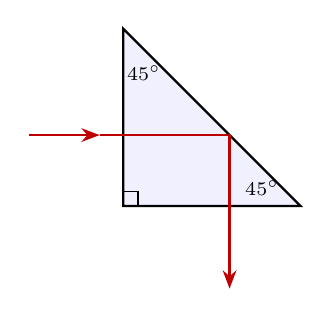
\begin{tikzpicture}[x=0.75cm,y=0.75cm,>=Stealth,font=\small]
  \draw[thick,fill=blue!6] (0,0) -- (3,0) -- (0,3) -- cycle;
  \draw[thick,red!75!black,->] (-1.6,1.2) -- (-0.4,1.2);
  \draw[thick,red!75!black] (-0.4,1.2) -- (1.8,1.2);
  \draw[thick,red!75!black,->] (1.8,1.2) -- (1.8,-1.4);
  \draw (0.25,0) -- (0.25,0.25) -- (0,0.25);
  \node[font=\scriptsize] at (2.35,0.3) {$45^\circ$};
  \node[font=\scriptsize] at (0.35,2.25) {$45^\circ$};
\end{tikzpicture}
\end{minipage}

%--------------------------------------------------------------------
\newpage
\begin{enumerate}[start=4]
\item \textbf{Képszerkesztés.} Az ábrákon egy négyzet $1$~cm, a tárgy $1{,}5$~cm magas. Az
  a)--c) ábrán gyűjtőlencse ($f = 2$~cm), a d) ábrán szórólencse ($f = -2$~cm) van.
  Szerkeszd meg a képet két nevezetes sugármenettel! Olvasd le a kép helyét és nagyságát,
  jellemezd a képet (valódi/látszólagos, állás, nagyítás), majd ellenőrizd a leképezési
  törvénnyel!
\end{enumerate}

\vspace{2pt}
\begin{center}
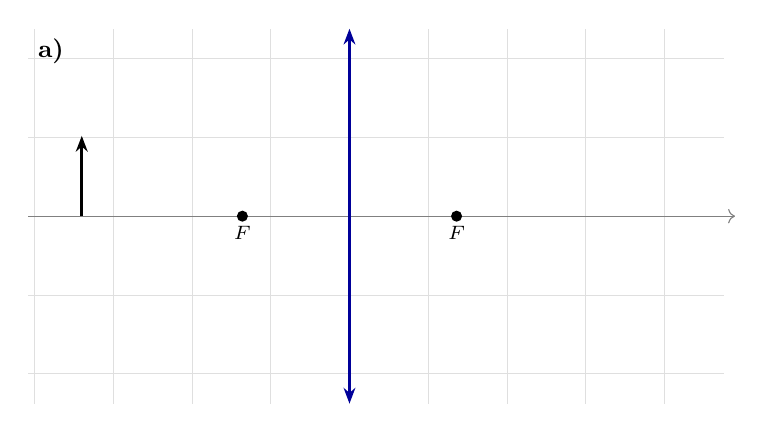
\begin{tikzpicture}[x=0.68cm,y=0.68cm]
  \ures{2}{5}{1.5}
  \node[anchor=north west,font=\small\bfseries] at (-6,3.5) {a)};
\end{tikzpicture}\hfill
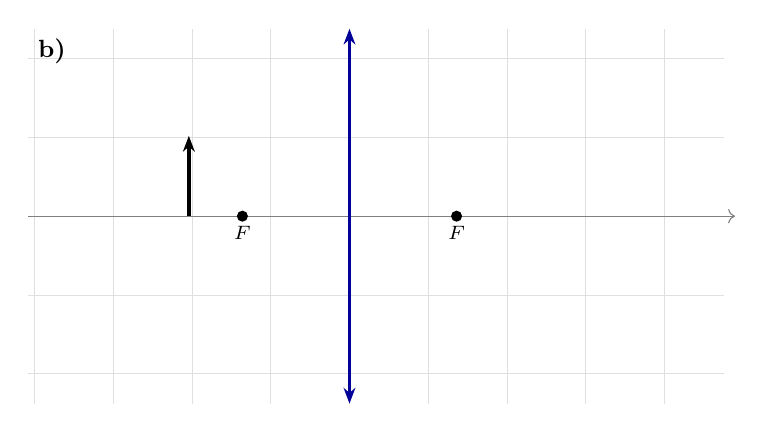
\begin{tikzpicture}[x=0.68cm,y=0.68cm]
  \ures{2}{3}{1.5}
  \node[anchor=north west,font=\small\bfseries] at (-6,3.5) {b)};
\end{tikzpicture}

\vspace{6pt}
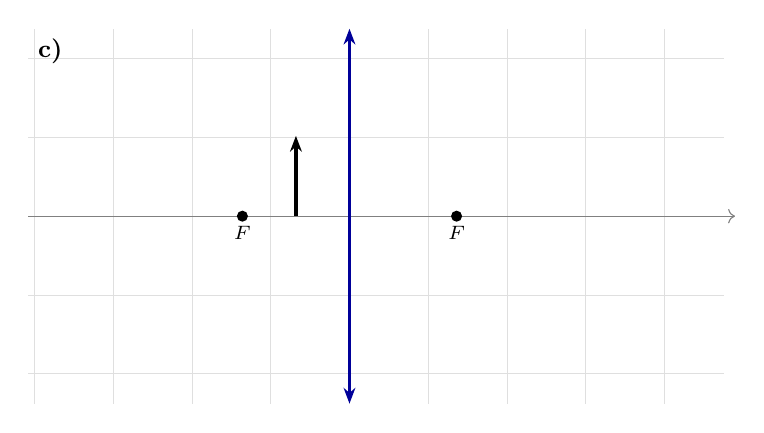
\begin{tikzpicture}[x=0.68cm,y=0.68cm]
  \ures{2}{1}{1.5}
  \node[anchor=north west,font=\small\bfseries] at (-6,3.5) {c)};
\end{tikzpicture}\hfill
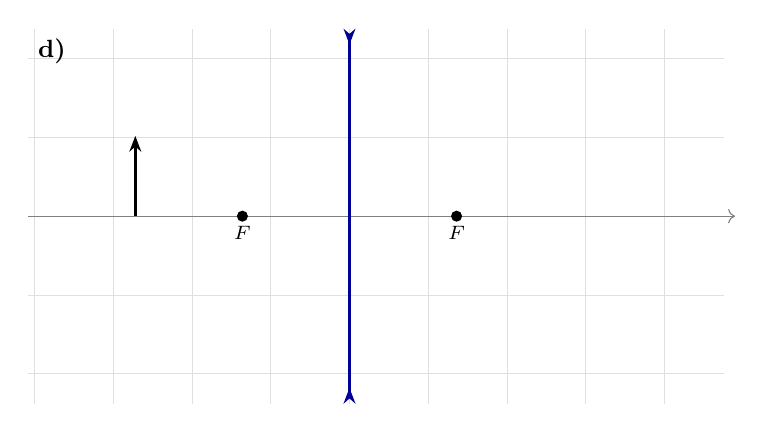
\begin{tikzpicture}[x=0.68cm,y=0.68cm]
  \ures{-2}{4}{1.5}
  \node[anchor=north west,font=\small\bfseries] at (-6,3.5) {d)};
\end{tikzpicture}
\end{center}

%--------------------------------------------------------------------
\newpage
\begin{enumerate}[start=5]
\item \textbf{Gyűjtőlencse.} Egy $f = 20$~cm fókusztávolságú gyűjtőlencse elé $5$~cm magas
  tárgyat teszünk.
  \begin{enumerate}
    \item Hány dioptriás a lencse? Hol keletkezik a kép, és mekkora, ha a tárgy $60$~cm-re
      van a lencsétől? Hova kell tenni az ernyőt, hogy a kép éles legyen?
    \item Hol keletkezik a kép, és mekkora, ha a tárgy $15$~cm-re van? Felfogható-e ernyőn?
    \item Hova tegyük a tárgyat, hogy ernyőn \textbf{négyszeres} nagyítású képet kapjunk?
      Hasonlítsd össze a b) esettel!
    \item A lencse kétszer domború, két lapjának görbületi sugara egyenlő, anyaga üveg.
      Mekkora a görbületi sugár? Mekkora lesz a lencse fókusztávolsága, ha víz alá
      merítjük? Gyűjtőlencse marad?
    \item Víz alatt egy kétszer domború alakú \textbf{légbuborék} is lencseként viselkedik.
      Gyűjtő- vagy szórólencse? (Számolás nélkül, a formula előjeléből döntsd el!)
  \end{enumerate}

\item \textbf{Vetítő és fényképezőgép.}
  \begin{enumerate}
    \item Egy diavetítő objektívjének fókusztávolsága $10$~cm, a vászon a lencsétől $5{,}1$~m-re
      van. Milyen messze van a dia a lencsétől? Mekkora a nagyítás, és mekkora lesz a
      vásznon egy $24~\text{mm} \times 36~\text{mm}$-es kép?
    \item A vásznat közelebb, a lencsétől $3{,}1$~m-re tesszük. Merre és mennyivel kell
      elmozdítani az objektívet a diához képest, hogy a kép újra éles legyen? Hogyan
      változik a kép mérete?
    \item Egy $f = 50$~mm-es fényképezőgéppel egy $5$~m-re álló, $1{,}8$~m magas embert
      fényképezünk. Milyen messze kell lennie az érzékelőnek a lencsétől? Ráfér-e az ember
      képe a $24~\text{mm} \times 36~\text{mm}$-es érzékelőre? Miért van távoli tárgyaknál az
      érzékelő szinte pontosan a fókuszsíkban?
  \end{enumerate}

\item \textbf{Tárgy és ernyő.} Egy gyertya és egy ernyő egymástól $90$~cm-re van. Közéjük
  egy $f = 20$~cm-es gyűjtőlencsét teszünk.
  \begin{enumerate}
    \item Hova kell tenni a lencsét, hogy az ernyőn éles kép legyen? (Két megoldás van!)
      Mekkora a nagyítás az egyes esetekben?
    \item Mekkora az a legkisebb tárgy--ernyő távolság, amelynél ezzel a lencsével még éles
      képet kaphatunk az ernyőn? (Segítség: mikor van megoldása a másodfokú egyenletnek?)
  \end{enumerate}
\end{enumerate}

%--------------------------------------------------------------------
\newpage
\begin{enumerate}[start=8]
\item \textbf{Tükrök.}
  \begin{enumerate}
    \item Egy kozmetikai tükör homorú, görbületi sugara $60$~cm. Milyen képet látunk benne,
      ha az arcunk $20$~cm-re van tőle? Hányszoros a nagyítás? Mi történik, ha $40$~cm-re
      hajolunk el tőle?
    \item Egy kereszteződésben elhelyezett domború tükör görbületi sugara $1$~m. Hol
      keletkezik, és mekkora egy tőle $10$~m-re álló, $4{,}5$~m hosszú autó képe? Miért
      domború tükröt használnak itt, és nem síktükröt?
    \item Legalább milyen magas síktükör kell ahhoz, hogy egy $170$~cm magas ember tetőtől
      talpig lássa magát benne? Függ-e ez attól, milyen messze áll a tükörtől?
      (Segítség: rajzold meg a fejtetőről és a talpról a szembe jutó sugarakat!)
  \end{enumerate}

\item \textbf{A szem és a szemüveg.}
  \begin{enumerate}
    \item Egy rövidlátó ember távolpontja $40$~cm. Milyen fókusztávolságú, hány dioptriás
      szemüveg kell neki? Gyűjtő- vagy szórólencse?
    \item Egy idős ember közelpontja $1$~m, de $25$~cm-ről szeretne olvasni. Milyen szemüveg
      kell neki? (A szemüveg a $25$~cm-re lévő betűkről $1$~m-re lévő látszólagos képet
      készítsen.)
    \item Egy $f = 5$~cm-es nagyítóval úgy nézünk egy bélyeget, hogy a látszólagos kép
      $25$~cm-re legyen a lencsétől. Hova kell tenni a bélyeget, és mekkora a nagyítás?
  \end{enumerate}

\item \textbf{Szóbeli gyakorlás.} Válassz egyet, és fejtsd ki összefüggő szövegben, 3--4
  percben: \textbf{(A)} \emph{A fénytörés} (törési törvény, törésmutató és terjedési
  sebesség, teljes visszaverődés, határszög, színszóródás, alkalmazások), vagy
  \textbf{(B)} \emph{Leképezés lencsékkel és gömbtükrökben} (fajták, fókusz, nevezetes
  sugármenetek, valódi és látszólagos kép, leképezési törvény, nagyítás, a szem és az
  optikai eszközök).
\end{enumerate}

\end{document}
